\documentclass{beamer}

\usepackage[T1]{fontenc}
\usepackage[utf8]{inputenc}
\usepackage[portuges]{babel}
\usepackage{amssymb,amsmath,amsrefs}
\usepackage{hyperref}
\usepackage{graphicx}

\newcommand{\p}{\partial}

\title{Escrita colaborativa com Git}
\author[KONZEN,AZEVEDO,GUIDI,JUSTO,SAUTER]{P.H.A.~Konzen \and F.S.~Azevedo \and L.F.~Guidi \and D.A.R.~Justo \and E.~Sauter}
\institute[IME-UFRGS]{Instituto de Matemática e Estatística\\
Universidade Federal do Rio Grande do Sul}
\date[XVIII Salão de Extensão]{XVIII Salão de Extensão\\16-19 de outubro de 2017\\Porto Alegre, RS\\UFRGS}

\begin{document}

\frame{\titlepage}

\begin{frame}{Sumário}
  \tableofcontents
\end{frame}

\section{Introdução}
\begin{frame}{Introdução}
  \begin{center}
    Escrita colaborativa é a criação de textos de modo colaborativo, supervisionado ou não por um grupo de organizadores~\cite{Wiki2017a}.
  \end{center}
  \begin{itemize}
  \item Exemplos de projetos:
    \begin{itemize}
    \item Wikipédia
    \item Cursos da Software Carpentry
    \item Projetos de ficção colaborativa:
      \begin{itemize}
      \item  Carvens, A Million Penguins, ...
      \end{itemize}
    \end{itemize}
  \end{itemize}
\vspace{1cm}
\begin{minipage}[hb!]{1.0\linewidth}
\hrule
\begin{bibdiv}
  \begin{biblist*}
    \bib{Wiki2017a}{misc}{
      author = {Wikipédia},
      title = {Escrita colaborativa --- Wikipédia{,} a enciclopédia livre},
      year = {2017},
      url = {\url{https://pt.wikipedia.org/w/index.php?title=Escrita_colaborativa&oldid=49878436}},
      note = {[Online; accessed 17-setembro-2017]}
    }
  \end{biblist*}
\end{bibdiv}
\end{minipage}
\end{frame}

\begin{frame}{Cálculo Numérico - Um livro colaborativo}
  \begin{center}
    \url{https://ufrgs.br/numerico}

    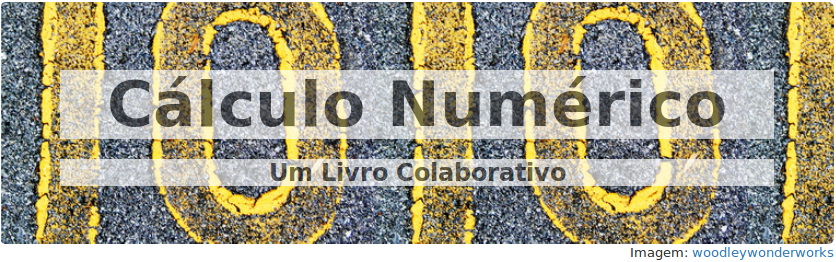
\includegraphics[scale=0.35]{./figs/Webpage_jumbotron.png}
  \end{center}
\end{frame}

\begin{frame}{Ferramentas necessárias}
  \begin{itemize}
  \item Licença compatível (Ex. CC-BY-SA 3.0)
    \begin{itemize}
    \item Direitos autorais
    \item Direitos de distribuição
    \item Direitos de cópia, adaptações, derivações, etc ...
    \end{itemize}
  \item Sistema de controle de versão
    \begin{itemize}
    \item Git (Repositórios {\it online} GitHub, GitLab, etc...)
    \item BitKeeper
    \item Mercurial
    \item Apache Subversion
    \item Wikipedia (solução própria)
    \item Authorea (solução própria)
    \item etc ...
    \end{itemize}
  \end{itemize}
\end{frame}

\begin{frame}{Git - controlador de versão}
  \begin{itemize}
  \item Sobre~\cite{Wiki2017b}:
    \begin{itemize}
    \item Abril, 2015 - Criado por Linus Torvalds$^+$
    \item Licença GNU General Public License (GPL e LGPL)
    \item Compatibilidade:
      \begin{itemize}
      \item Linux
      \item BSD
      \item Windows
      \item entre outras ...        
      \end{itemize}
    \item Versatilidade:
      \begin{itemize}
      \item Repositórico armazenado localmente
      \item Histórico completo das versões
      \item Acompanhamento local de versões
      \end{itemize}
    \end{itemize}
  \end{itemize}
  \begin{itemize}
  \item Hospedagem de código
    \begin{itemize}
    \item {\bf GitHub}
    \item Sourceforge
    \item GitLab
    \item entre outros ...
    \end{itemize}
  \end{itemize}
  \vspace{0.25cm}
  \begin{minipage}[hb!]{1.0\linewidth}
    \hrule
    \begin{bibdiv}
      \begin{biblist*}
        \bib{Wiki2017b}{misc}{
          author = {Wikipédia},
          title = {Git --- Wikipédia{,} a enciclopédia livre},
          year = {2017},
          url = {\url{https://pt.wikipedia.org/w/index.php?title=Git&oldid=49331936}},
          note = {[Online; accessed 18-julho-2017]}
        }
      \end{biblist*}
    \end{bibdiv}
  \end{minipage}
\end{frame}

\section{Colaborando com um projeto no {\bf Git}Hub}

\begin{frame}{Criando uma conta no {\bf Git}Hub}
  \begin{center}
    {\bf Git}Hub é uma plataforma de hospedagem de código-fonte que permite o gerenciamento de projetos públicos de forma gratuíta. O sistema de controle de versão é o {\bf Git}.
  \end{center}
  \begin{center}
    \url{https://github.com/}
    
    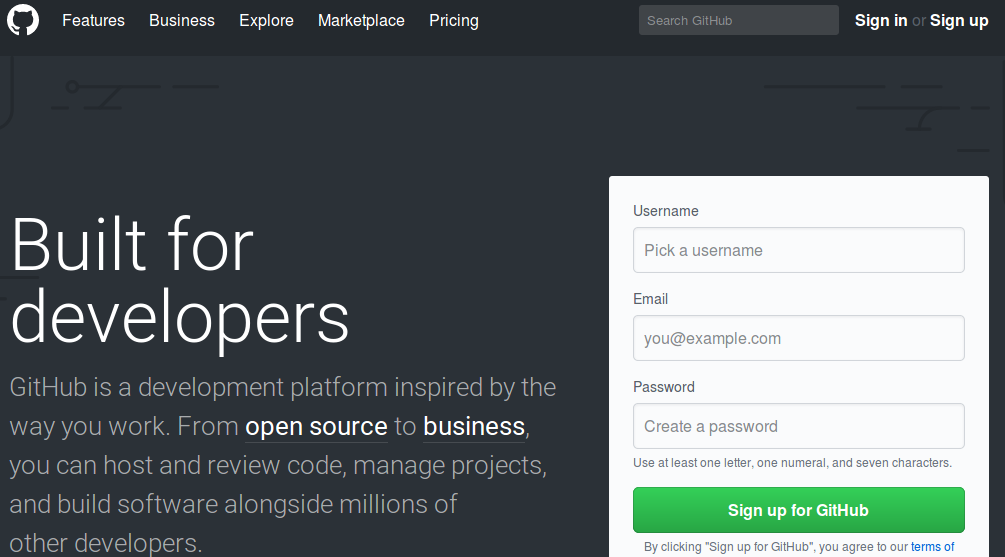
\includegraphics[scale=0.25]{./figs/SignUp_GitHub.png}
  \end{center}
\end{frame}

\begin{frame}{{\it Fork us on GitHub!}}
  \begin{center}
    \url{https://github.com/livroscolaborativos/Oficina}

    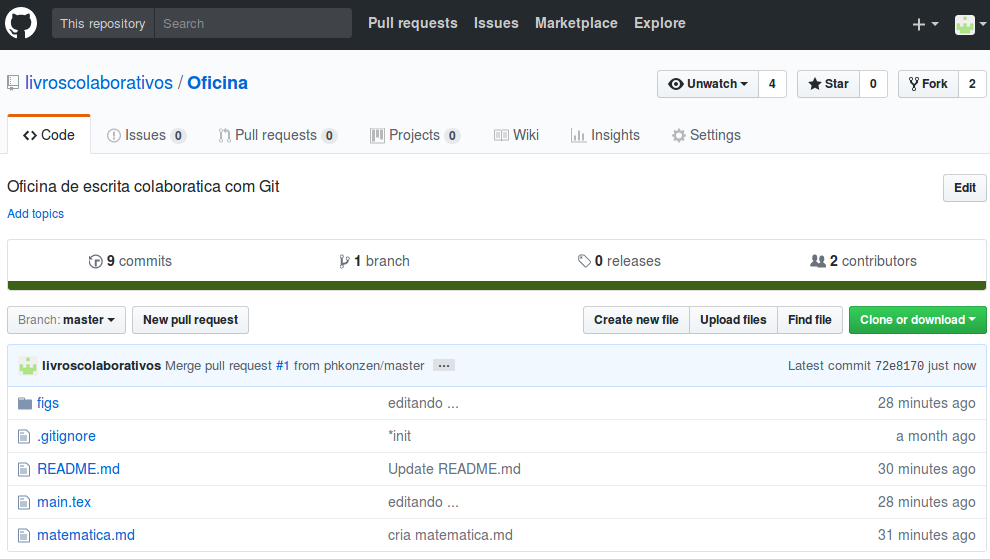
\includegraphics[scale=0.3]{./figs/Fork_us_on_GitHub.png}
  \end{center}
\end{frame}

\begin{frame}{Participe da escrita do texto}
  \begin{center}
    https://github.com/{\bf USUARIO}/Oficina/blob/master/matematica.md

    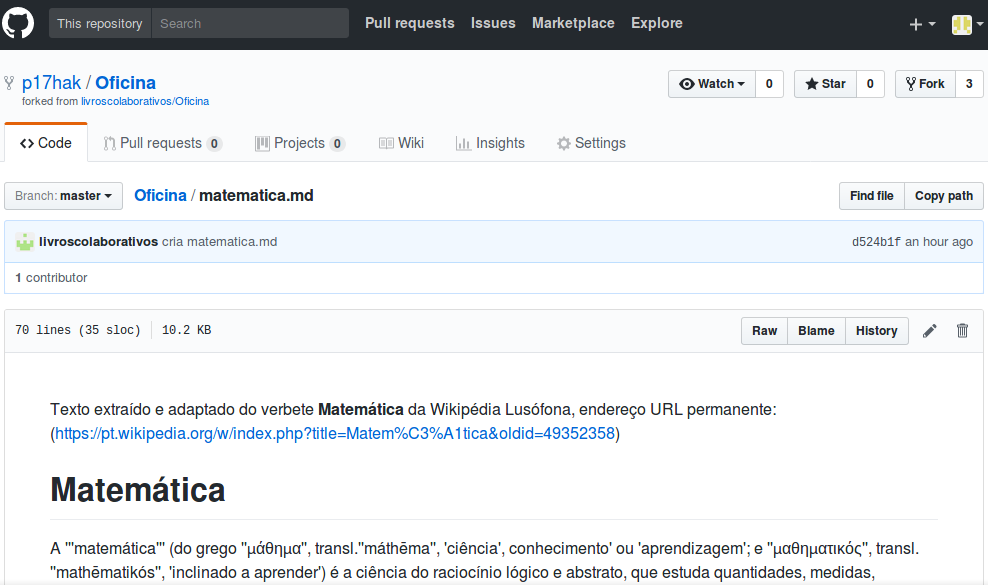
\includegraphics[scale=0.3]{./figs/matematica_GitHub.png}
  \end{center}
\end{frame}

\begin{frame}{Editando o texto}
  \begin{center}
    https://github.com/{\bf USUARIO}/Oficina/edit/master/matematica.md

    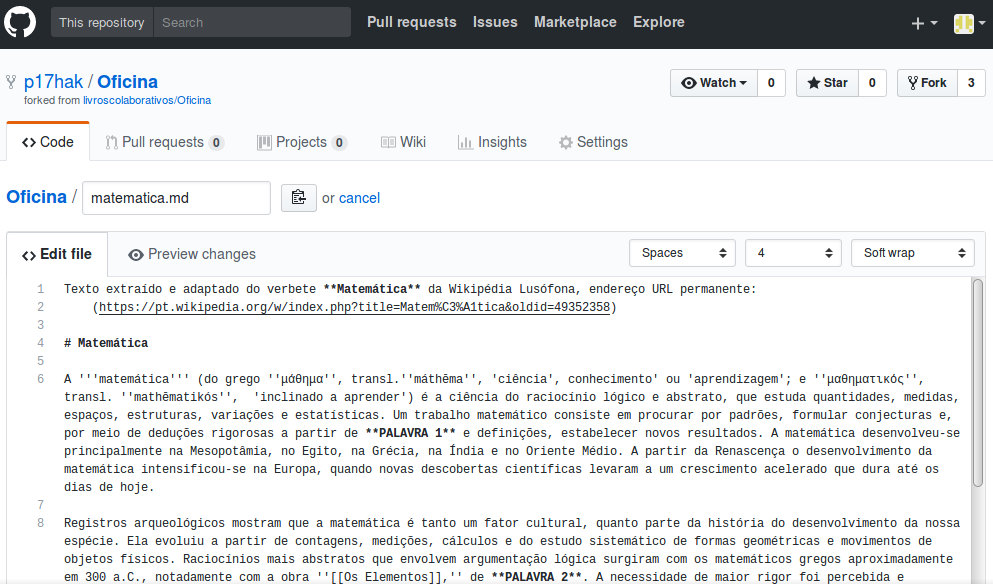
\includegraphics[scale=0.3]{./figs/editando_GitHub.png}
  \end{center}
\end{frame}

\begin{frame}{{\it commit} - Registrando sua versão}
  \begin{center}
    https://github.com/{\bf USUARIO}/Oficina/edit/master/matematica.md

    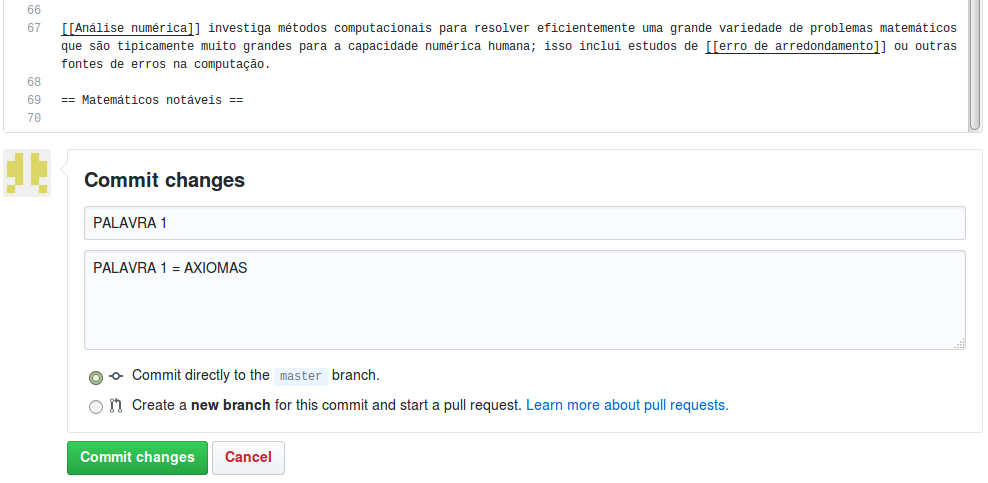
\includegraphics[scale=0.3]{./figs/commit_GitHub.png}
  \end{center}
\end{frame}

\begin{frame}{{\it New Pull request} - Enviando sua versão}
  \begin{center}
    https://github.com/{\bf USUARIO}/Oficina

    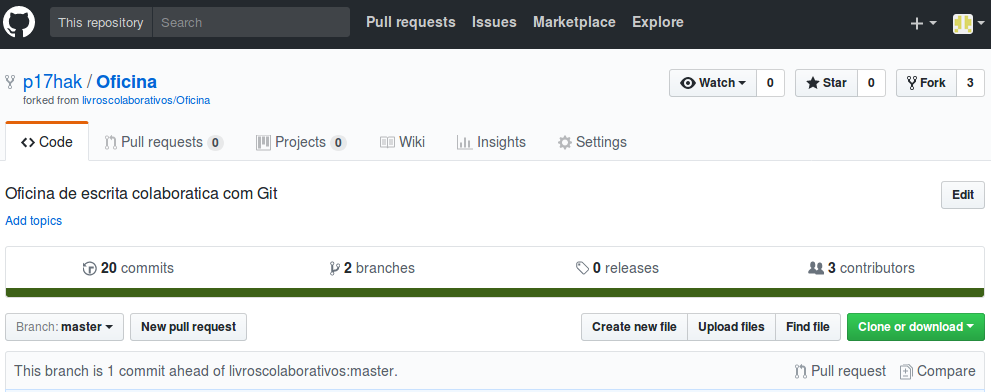
\includegraphics[scale=0.3]{./figs/New_pull_request_GitHub.png}
  \end{center}
\end{frame}

\begin{frame}{Registrando sua requisição}
  \begin{center}
    https://github.com/{\bf livroscolaborativos}/Oficina

    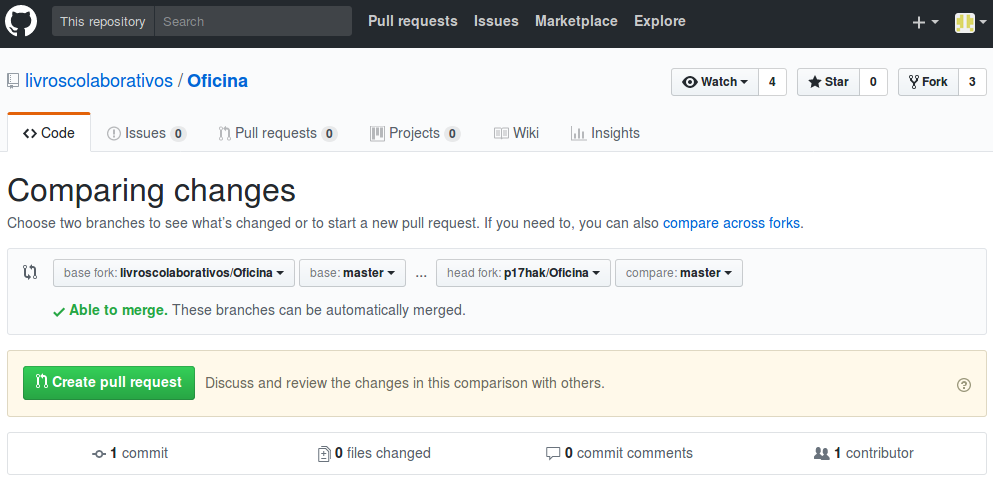
\includegraphics[scale=0.3]{./figs/Create_pull_request_GitHub.png}
  \end{center}
\end{frame}

\begin{frame}{Registrando sua requisição}
  \begin{center}
    https://github.com/{\bf livroscolaborativos}/Oficina

    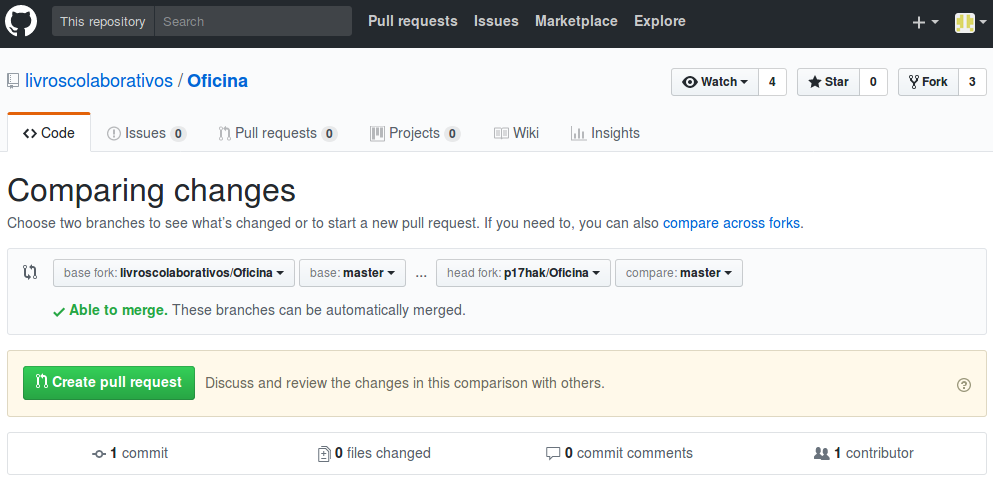
\includegraphics[scale=0.3]{./figs/Create_pull_request_GitHub.png}
  \end{center}
\end{frame}

\begin{frame}{Um conflito!}
  \begin{center}
    https://github.com/{\bf livroscolaborativos}/Oficina

    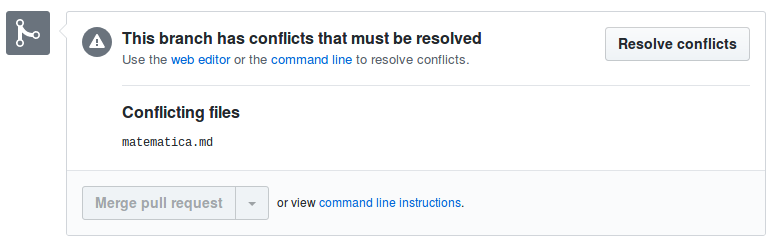
\includegraphics[scale=0.3]{./figs/Conflict_GitHub.png}
  \end{center}
\end{frame}

\begin{frame}{Resolvendo um conflito!}
  \begin{center}
    https://github.com/{\bf livroscolaborativos}/Oficina

    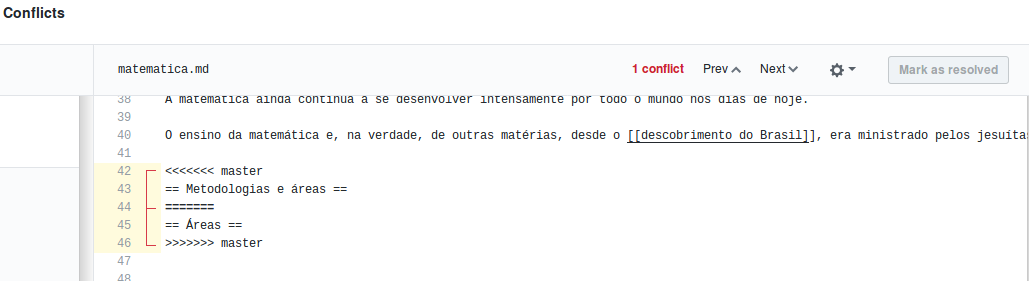
\includegraphics[scale=0.3]{./figs/Mark_as_resolved_GitHub.png}
  \end{center}
\end{frame}

\begin{frame}{Atualizando seu Fork}
  \begin{center}
    https://github.com/{\bf USUÁRIO}/Oficina

    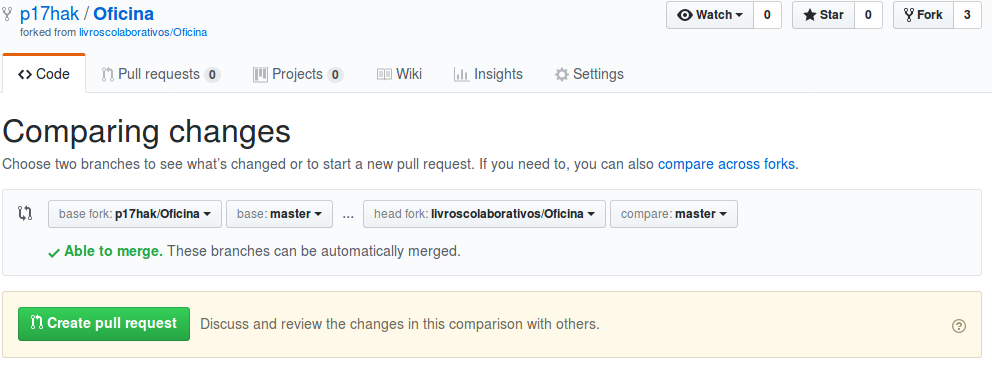
\includegraphics[scale=0.3]{./figs/Sync_GitHub.png}
  \end{center}
\end{frame}


\begin{frame}{Comece seu próprio projeto}
  \begin{center}
    \url{https://github.com/dashboard}
    
    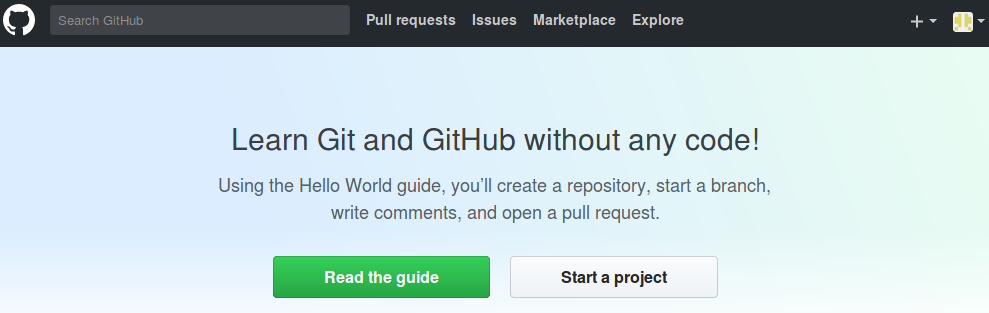
\includegraphics[scale=0.3]{./figs/Start_a_project_GitHub.png}
  \end{center}
\end{frame}

\begin{frame}{{\bf Fork us on GitHub!}}
  \begin{center}
    Não deixe de participar da escrita do

    {\Large Cálculo Numérico - Um Livro Colaborativo}

    \url{https://github.com/livroscolaborativos/CalculoNumerico}
  \end{center}
  \vspace{1cm}
  \begin{center}
    {\Huge Tenham ótimas colaborações!}
  \end{center}
\end{frame}


\end{document}